
\documentclass[12pt]{article}%
\usepackage{amsfonts}
\usepackage{amsmath}
\usepackage[a4paper, top=2.5cm, bottom=2.5cm, left=2.2cm, right=2.2cm]%
{geometry}
\usepackage{times}
\usepackage{complexity}
\usepackage{graphicx}
\usepackage{physics}
\usepackage{amsmath}
\usepackage{amssymb}
\newenvironment{proof}[1][Proof]{\textbf{#1.} }{\ \rule{0.5em}{0.5em}}

\begin{document}

\title{ECE 621 HW 2}
\author{Edward Kim}
\date{\today}
\maketitle

\section*{Problem 1}
\begin{enumerate}
	\item The inverse of $g$ would be $g^{-1} = c \cdot b \cdot a$
	\item For $K = \langle a \rangle$, this would simply be the subset $\{e, a \}$ where $e$ is the identity element of group $G$. Multiplying all of these elements shows that this set is closed under the group operation. For $H = \langle a, b \rangle $, a direct calculation shows the elements of $H$ can be expressed as the set \( \{e, a ,b , ab, ba, aba, bab, \cdots \} \). By the assumption that the generating elements $a,b$ are self-inverses, we can reason that the multiplication of alternating elements result in alternating elements.
	\item Under bitwise addition modulo two, each of the elements $001, 010, 100$ are self-inverses. Furthermore, it is evident that each element is distinct and a pair cannot generate the remaining other. Since these elements generate all three bit strings, $|G| = 2^3 = 8$. Similarly, $|H| = 2^2 = 4$ and $|K| = 2$.
	\item The Pauli matrices have the relation $XZ = -iY, XY = iZ, YZ = -iX$. Adddtionally, all pairs of the Pauli matrices anti-commuate. By iterating all of the possible products of the Pauli matrices $X,Y,Z$, the group generated will be the set:
	\[ \{ \pm I,\pm iI, \pm X, \pm iX, \pm Y, \pm iY, \pm Z, \pm iZ \} \]	
For the subgroups $H,K$, \[ H = \langle X, Y \rangle = \langle X, iXZ \rangle  = \langle X, Y, iZ \rangle =  G\] 
and \[ K = \langle X \rangle = \{ I, X \} \]
showing that $|G| = |H| = 16$ and \(|K| = 2\) 
\item This is a consequence of having elements of your generating group having a dependence relationship of one another. A group with a generating set could have multiple such generating sets as a result.
\item $G$ could have infinite order.
\item Take \(a = X \otimes X, b = Y \otimes Y, c = Z \otimes Z\) and the identity to be \(I \otimes I\)  
\end{enumerate}
\section*{Problem 2}
\begin{enumerate}
	\item From our derivations, we know that channel capacity of the 10\% binary symmetric channel is $1 - H_b(\frac{1}{10}) \approx 1 - 0.325 = 0.675$ 
	\item 
		\begin{description}
			\item[Triple Modular Redundancy Code:] Since this code can correct one bit error in each block, a successful decode would mean each a successful decode of each block. The probability that a codeword can be successfully decoded is:
				\begin{equation*}
					p_0 = \left(\left(\frac{9}{10}\right)^3 + 3\left(\frac{1}{10}\right)\left(\frac{9}{10}\right)^2\right)^3 
				\end{equation*}
			\item[Hamming Code:] Suppose that out Hamming code generator matrix is the canonical form \( G =  \left(\begin{matrix} I_{4\times 4} \\ A \end{matrix} \right)\) . Since the $4^{th}$ bit of the codeword will always be correct (since Bob has access to the information that the $4^{th}$ bit will be set to zero), it suffices to calculate the probability of successful decoding by considering the probability that at most one error will occur on the remaining bits:
				\begin{equation*}
					p_1 = \left(\frac{9}{10}\right)^6 + 6\left(\frac{1}{10}\right)\left(\frac{9}{10} \right)^5
				\end{equation*}
			\item[Dual Hamming Code:] The dual Hamming code can also correct at most one bit error:
				\begin{equation*}
					p_2 = \left(\frac{9}{10}\right)^7 + 7\left(\frac{1}{10}\right)\left(\frac{9}{10} \right)^6 
				\end{equation*}
		\end{description}
		The average probability would be \(\frac{p_0 + p_1 + p_2}{3} \) 
\end{enumerate}

\section*{Problem 3}
\begin{enumerate}
	\item The Pauli matrix representations of the channels can be found first noting the following equivalences:
		\begin{description}
			\item[Ampitude Damping Channel: ] 
				\begin{align*}
					\label{eq:}
					A_0 & = \left(\begin{matrix} 1 & 0 \\ 0 & \sqrt{1-p} \end{matrix}\right) = \frac{1 + \sqrt{1 - p}}{2}I + \frac{1 - \sqrt{1-p}}{2} Z \\
					A_1 & = \left(\begin{matrix} 0 &  \sqrt{p} \\ 0 & 0  \end{matrix} \right) = \frac{\sqrt{p}}{2} \left(X + iY \right)   
				\end{align*}
			\item[Phase Damping Channel:] 
				\begin{align*}
					A_0 & = \left(\begin{matrix} \sqrt{1-p} & 0 \\ 0 & \sqrt{1-p} \end{matrix}\right) = \sqrt{1-p}I \\
					A_1 & = \left(\begin{matrix} \sqrt{p} & 0 \\ 0 & 0 \end{matrix}\right) = \frac{\sqrt{p}}{2} (I + Z) \\
					A_2 & = \left(\begin{matrix} 0 & 0 \\ 0 & \sqrt{p} \end{matrix}\right) = \frac{\sqrt{p}}{2} (I- Z) 
				\end{align*}
		\end{description}
		Expanding the Kraus operator representations \(A_r \rho A_r^{\dagger} \) in terms of the equivalences above and taking the adjoint as needed gives us the required Pauli matrix representation for both channels.
	\item From our observations above, we expand the Pauli matrix representation as follows:
		\begin{align*}
			A_0 \rho A_0^\dagger + 	A_1 \rho A_1^\dagger 	+ A_2	 \rho A_2^\dagger & = (1-p)\rho + \frac{p}{4}(I+Z)\rho(I+Z)^\dagger + \frac{p}{4} (I - Z) \rho (I-Z)^\dagger \\
													& = 1 - p\rho + \frac{p}{2} \rho + \frac{p}{2} Z\rho Z = (1 - \frac{p}{2})\rho + \frac{p}{2} Z\rho Z
		\end{align*}
		By setting $q = \frac{p}{2} $, we see that the channel applies the Z operator with probability \(q\)  and leaves it untouched with probabilty $1 - q$ 
		.\item 
		We can use Stinespring Dilaton to construct the following isometries which respect the evolution governed by the Quantum Channel:
		\begin{description}
			\item[Amplitude Damping Channel] 
				\begin{equation*}
					U = A_0 \otimes \ket{0} + A_1 \otimes \ket{1} =  \left(\begin{matrix} 1 & 0 \\ 0 & \sqrt{1-p} \end{matrix}\right) \otimes \ket{0} +  \left(\begin{matrix} 0 &  \sqrt{p} \\ 0 & 0  \end{matrix} \right) \otimes \ket{1}  
				\end{equation*}
			\item[Phase Damping Channel] 
				\begin{align*}
					U & = A_0 \otimes \ket{0} + A_1 \otimes \ket{1} + A_2 \otimes \ket{2} \\ 
						& = \left(\begin{matrix} \sqrt{1-p} & 0 \\ 0 & \sqrt{1-p} \end{matrix}\right) \otimes \ket{0} \\
						& + \left(\begin{matrix} \sqrt{p} & 0 \\ 0 & 0 \end{matrix}\right) \otimes \ket{1} \\ 
						& +	\left(\begin{matrix} 0 & 0 \\ 0 & \sqrt{p} \end{matrix}\right) \otimes \ket{2}
				\end{align*}
		\end{description}
		By expanding the domain Hilbert space to include the enviroment (initialized to $\ket{0}$), the unitaries must extend the isometry defined above for both channels which leads to requirements:
		\begin{description}
			\item[Amplitude Damping Channel:] 
			\begin{gather*}
			\tilde{U}(\ket{0}\otimes \ket{0}) = \ket{0} \otimes \ket{0} \\
			\tilde{U}(\ket{1}\otimes \ket{0}) = \sqrt{1-p} \ket{1} \otimes \ket{0} + \sqrt{p} \ket{0} \otimes \ket{1} \\
			\end{gather*}
			One such extension is:
			\[
				\tilde{U} = \left( \begin{matrix}
						1 & 0 & 0 & 0 \\
						0 & - \sqrt{1 - p} & \sqrt{p} & 0 \\
						0 & \sqrt{p} & \sqrt{1 - p} & 0 \\
						0 & 0 & 0 & 1
				\end{matrix}\right)
		\]
			\item[Phase Damping Channel] 
			\begin{gather*}
				\tilde{U}(\ket{0} \otimes \ket{0}) = \sqrt{1 -p} \ket{0} \otimes \ket{0} + \sqrt{p} \ket{0} \otimes \ket{1} \\
				\tilde{U}(\ket{1} \otimes \ket{0}) =  \sqrt{1-p} \ket{1} \otimes \ket{0} + \sqrt{p}\ket{1} \otimes \ket{2}
			\end{gather*}
		\end{description}
	\item The following quantum circuit implements the error channel:
		\begin{figure}[h]
			\centering
			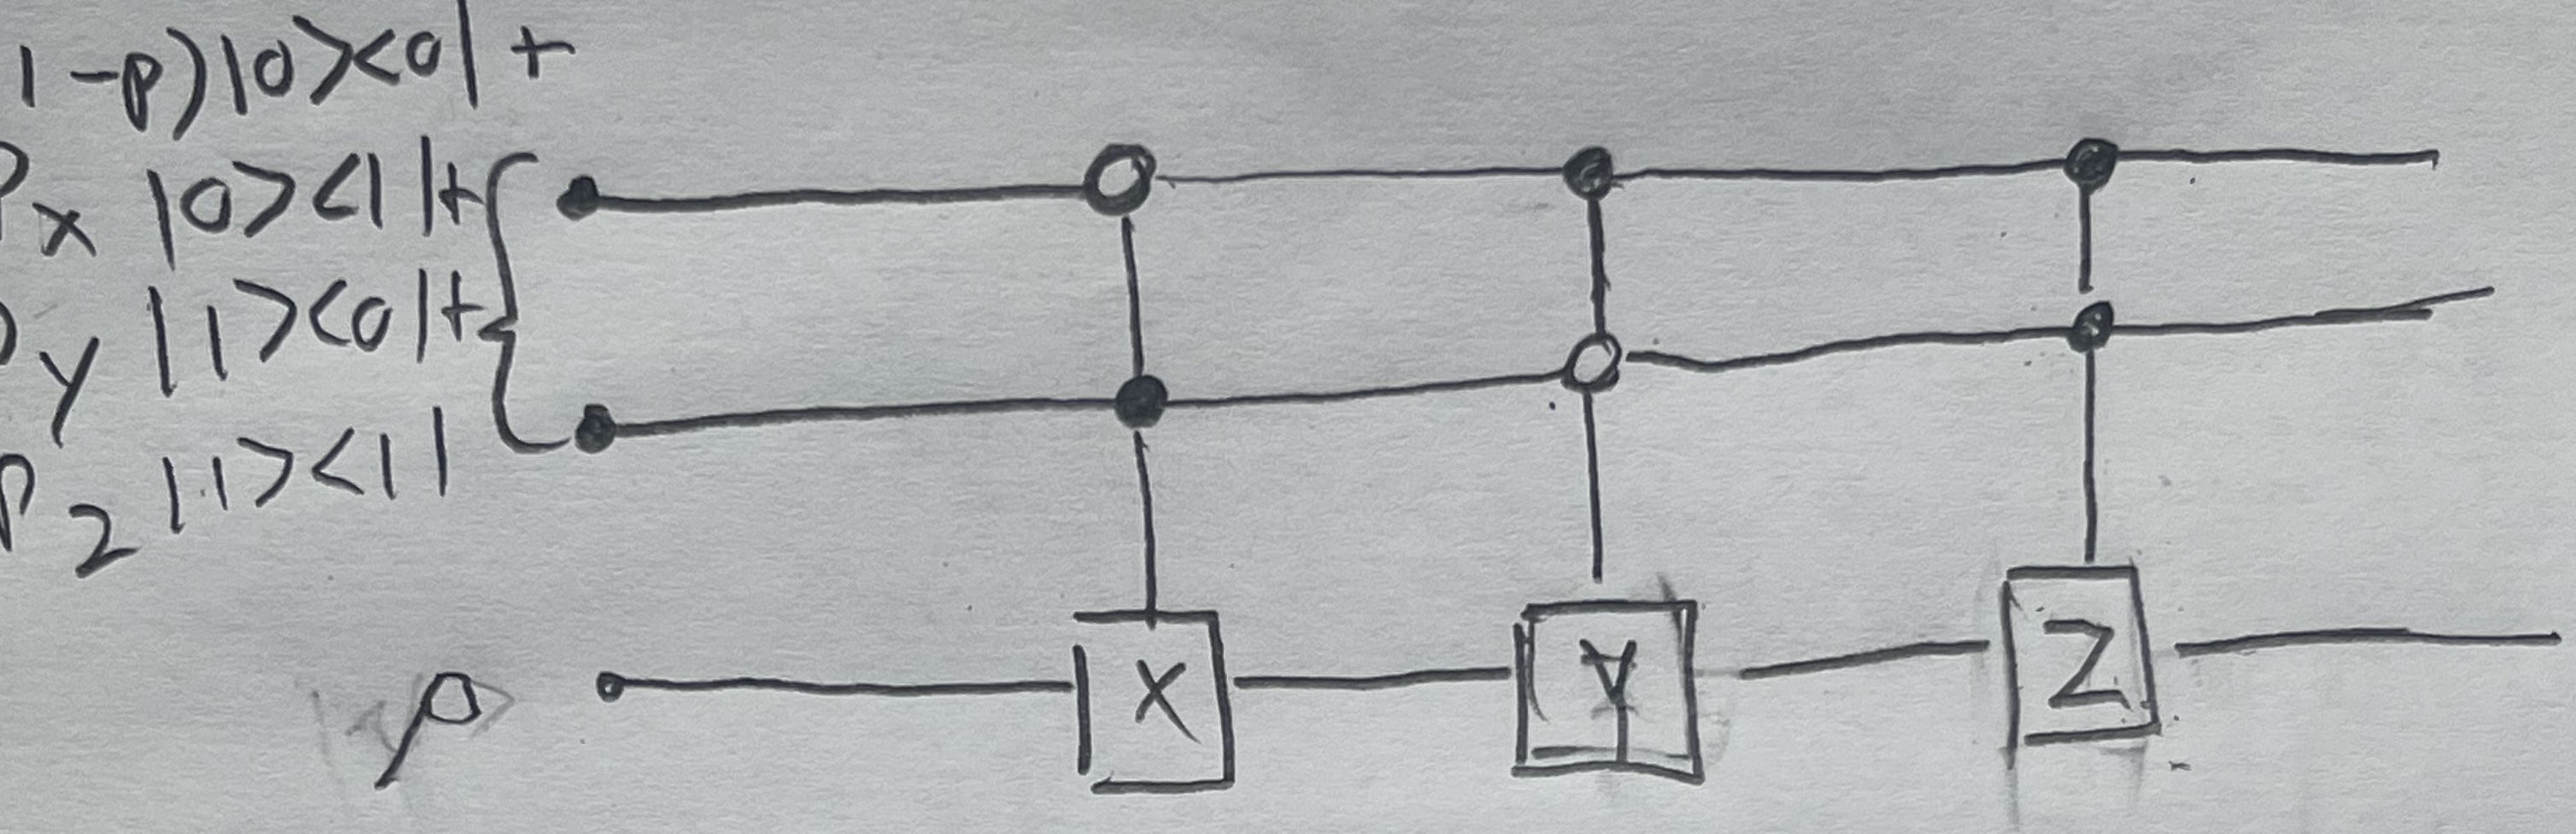
\includegraphics[width=0.8\textwidth]{fig}
			\caption{Error Circuit}
			\label{fig:}
		\end{figure}
where the two qubits above is a mixed state controlling the evolution of the input state below.
\end{enumerate}

\end{document}


